\documentclass{article}
% Set the font (output) encodings
\usepackage[LGR, T1]{fontenc}

% Language setting
% Replace `english' with e.g. `spanish' to change the document language
\usepackage[greek]{babel}

% Set page size and margins
% Replace `letterpaper' with `a4paper' for UK/EU standard size
\usepackage[letterpaper,top=2cm,bottom=2cm,left=3cm,right=3cm,marginparwidth=1.75cm]{geometry}

% Useful packages
\usepackage{amsmath}
\usepackage{graphicx}
\usepackage[colorlinks=true, allcolors=blue]{hyperref}
\usepackage{float}

\title{\textlatin{ChronoQuest}: Εκπαιδευτικό Λογισμικό 2025}

\author{
    Μαρία Δημητρούλη\\ \texttt{Π21028} \and 
    Κωνσταντίνος Σκλαβενίτης\\ \texttt{Π21151} \and 
    Γιώργος Νικολαΐδης\\ \texttt{Π21115}}
\begin{document}
\maketitle

% To add a section, create a new .tex file under /sections!

\section{Εισαγωγή}
Το σύστημα "\textlatin{ChronoQuest}" είναι ένα διαδικτυακό λογισμικό που έχει στόχο την εκμάθηση χρηστών ως προς ένα πολιτισμικό ή τουριστικό θέμα. Για την επιδίωξη του στόχου αυτού, το σύστημα περιέχει:
\begin{itemize}
    \item \textbf{Ενότητες} εμπλουτισμένες με κείμενο και εικόνες, με σκοπό την ενίσχυση της αρχικής επαφής ή της επανάληψης του χρήστη με το θέμα
    \item \textbf{Κουίζ} με ερωτήσεις αυτοαξιολόγησης.
     \item \textbf{Ενισχυτικό Υλικό} που θα προσαρμόζεται με βάση τις ανάγκες του χρήστη. Σκοπός του είναι η προετοιμασία του χρήστη για το τελικό διαγώνισμα.
\end{itemize}

Για να θεωρηθεί ότι ο χρήστης έχει ολοκληρώσει ένα θέμα, θα πρέπει μαζί με τις ερωτήσεις κουίζ και την ανάγνωση των ενοτήτων να γράψει και ένα τελικό \textbf{διαγώνισμα} το οποίο θα καλύπτει όλες τις ενότητες του θέματος. Το διαγώνισμα θα είναι προσαρμοσμένο στις ιδιαιτερότητες του χρήστη, έτσι ώστε να μην νιώσει αδικημένος/-η και χαθεί το ενδιαφέρον.
\section{Προσαρμοσμένη Μάθηση}
\subsection{Μαθηματικός Ορισμός Μοντέλου Μάθησης}
Το \textlatin{ChronoQuest} θα έχει ένα σύστημα προσαρμοσμένης μάθησης. Η αρμοδιότητά του θα είναι η πιθανοτική αξιολόγηση με βάση τέσσερις παραμέτρους \cite{bkt_wiki}:
\begin{itemize}
    \item \textbf{$p_{init}(s)$}: Η πιθανότητα ο χρήστης να έχει γνώση πάνω σε κάποιο θέμα/ενότητα \textbf{$s$}.
    \item \textbf{$p_{learn}(s)$}: Η πιθανότητα ο χρήστης να μάθει το θέμα $s$ μετά από προσπάθεια
    \item \textbf{$p_{slip}(s)$}: Η πιθανότητα ο χρήστης να κάνει λάθος παρόλο τη γνώση του στο θέμα $s$
    \item \textbf{$p_{guess}(s)$}: Η πιθανότητα ο χρήστης να απαντήσει σωστά παρόλο τη έλλειψη γνώσης του στο συγκεκριμένο θέμα $s$
\end{itemize}

Οι παραπάνω παράμετροι είναι μέρος του αλγόριθμου γνωστού ως \textlatin{\textbf{Bayesian Knowledge Tracing (BKT)}}. Αυτός ο αλγόριθμος, με τη χρήση των τεσσάρων παραμέτρων, μας δίνει μια \textbf{πιθανότητα επιδεξιότητας} ενός χρήστη $u$ για ενα συγκεκριμένη θέμα $s$. Οι παρακάτω εξισώσεις μπορούν να εφαρμοστούν για την ενημέρωση του μοντέλου όταν αλληλεπιδρά ο χρήστης $u$:

(1) Αρχικοποίηση:
$$p(X_1, s, u) = p_{init}$$

(2) Υπό συνθήκη πιθανότητα όταν ο χρήστης απαντάει σωστά:
$$p(X_t\ |\ obs = correct, s, u) = \frac{p(X_t, s, u) \cdot (1 - p_{slip}(s))}{p(X_t,s,u) \cdot (1 - p_{slip}(s)) + (1 - p(X_t, s, u)) \cdot p_{guess}(s) }$$

(3) Υπό συνθήκη πιθανότητα όταν ο χρήστης απαντάει λάθος:
$$p (X_t\ |\ obs = wrong, s, u) = \frac{p(X_t, s, u) \cdot p_{slip}(s)}{p(X_t,s,u) \cdot p_{slip}(s) + (1 - p(X_t, s, u)) \cdot (1 - p_{guess}(s)) }$$

(4) Ενημέρωση της πιθανότητας επιδεξιότητας:
$$p(X_{t+1}, s, u) = p(X_t\ |\ obs, s, u) + (1 - p(X_t\ |\ obs, s, u)) \cdot p_{learn}(s)$$

(5) Πιθανότητα ο χρήστης να κατέχει την έννοια σε επόμενη αλληλεπίδραση:
$$p(C_{t+1}, s, u) = p(X_{t+1}, s, u) \cdot (1 - p_{slip}(s)) + (1 - p(X_{t+1}, s, u)) \cdot p_{guess}(s)$$

Το σύστημα προσαρμοσμένης μάθησης θα παίρνει αποφάσεις για ένα χρήστη με βάση την εξίσωση (5).

\subsection{Χρήση εντός του \textlatin{ChronoQuest}}

Το σύστημα \textlatin{BKT} που ορίστηκε παραπάνω, θα χρησιμοποιηθεί για την πρόβλεψη και την καταγραφή της απόδοσης του χρήστη στα διάφορα θέματα.

Ένα θέμα μπορεί να είναι η γεωγραφία του τόπου, ή η ιστορία του. Έτσι, η απόδοση του χρήστη θα αξιολογείται με βάσει αυτά τα θέματα. 

\subsection{Αλγόριθμος Υπολογισμού Απόδοσης}
Αν αποθηκεύσουμε κάθε πιθανότητα επιδεξιότητας που καταγράφεται του μοντέλου \textlatin{BKT} μπορούμε να κατασκευάσουμε ένα \textbf{ιστορικό επιδεξιότητας} του χρήστη για ένα θέμα.

\begin{figure}[H]
    \centering
    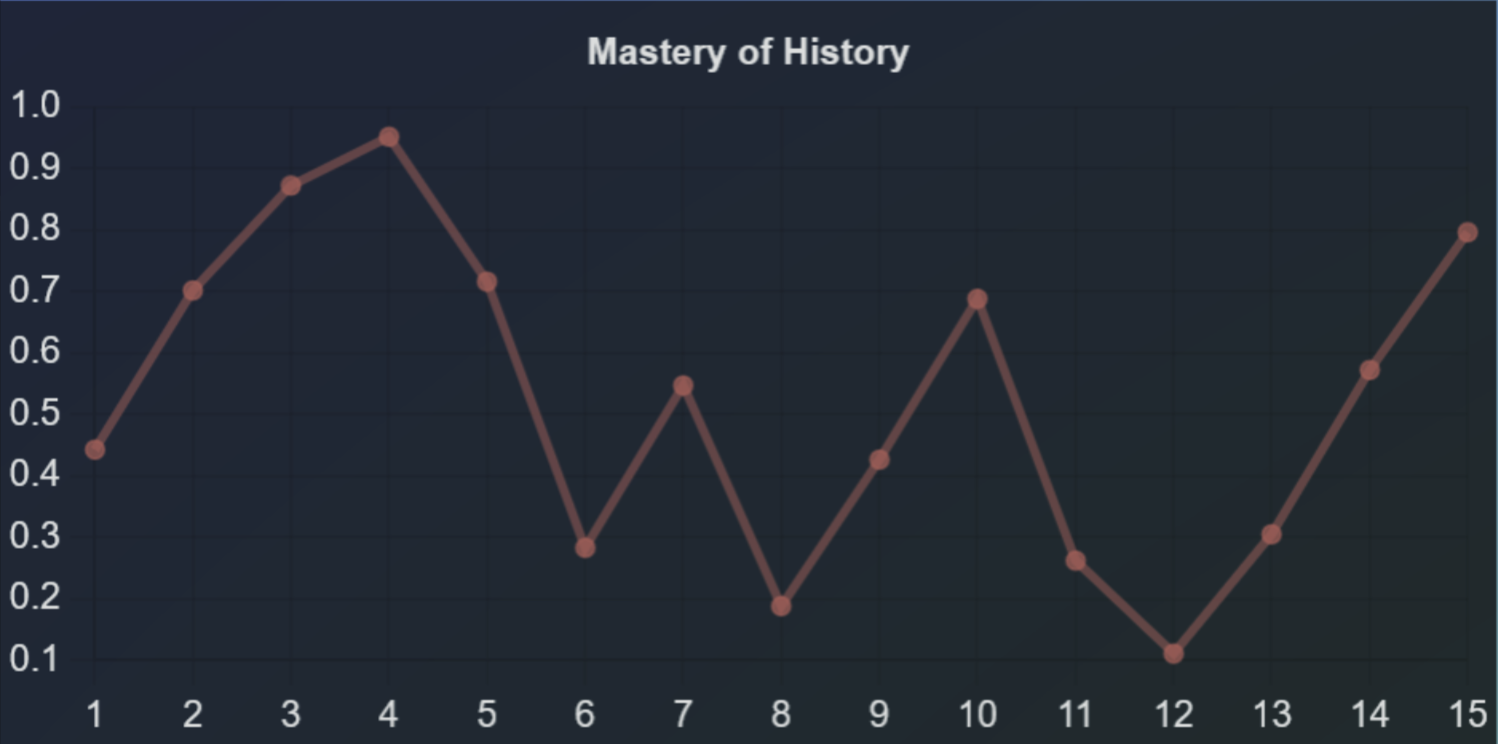
\includegraphics[width=0.5\linewidth]{img/MasteryGraph.png}
    \caption{Ιστορικό επιδεξιότητας}
\end{figure}

Ένας άνθρωπος μπορεί οπτικά μέσω του παραπάνω γραφήματος να βγάλει σωστά συμπεράσματα για την απόδοση του. Ας δούμε πως μπορούμε να "μαθηματικοποιήσουμε" την διαδικασία λήψης συμπερασμάτων.

Θα χρησιμοποιήσουμε 4 μετρικές για να αποκτήσουμε μια πολύ καλή εικόνα της απόδοσης του χρήστη:
\subsubsection{Ταχύτητα Μάθησης}
\subsubsection{Μοτίβα Απόκρισης}
\subsubsection{Αποδοτικότητα}
\subsubsection{Πρόοδος Μάθησης}

\section{Ανάλυση Απαιτήσεων}
Λειτουργικές απαιτήσεις ορίζουμε χαρακτηριστικά του συστήματος. Για ευκολία στην αναφορά μιας απαίτησης, κωδικοποιούμε την καθεμιά \textlatin{FR-XX-NNN}, όπου το \textbf{ΧΧ} είναι ένα πλαίσιο του πεδίου στο οποίο η απαίτηση αναφέρεται και το \textbf{NNN} είναι ο αριθμός της απαίτησης σχετικά με το πλαίσιο \textbf{ΧΧ}.

\subsection{Χρήστες}
\begin{itemize}
    \item \textbf{\textlatin{FR-USR-001}}: Ένας χρήστης θα μπορεί να συνδεθεί στο σύστημα με την χρήση του \textlatin{e-mail} και του κωδικού πρόσβασης του
    \item \textbf{\textlatin{FR-USR-002}}: Ένας χρήστης θα μπορεί να διαβάσει "θεωρία" για κάθε κεφάλαιο
    \item \textbf{\textlatin{FR-USR-003}}: Ένας χρήστης θα έχει τη δυνατότητα να απαντήσει στα κουίζ χωρίς περιορισμό (δεν απαιτείται να έχει πρώτα διαβάσει τη θεωρία)
    \item \textbf{\textlatin{FR-USR-004}}: Ένας χρήστης θα μπορεί να δει τα στατιστικά του
    \item \textbf{\textlatin{FR-USR-005}}: Ένας χρήστης θα μπορεί να γράφει διαγώνισμα όταν έχει ολοκληρώσει όλα τα κουίζ
\end{itemize}

\subsection{Ενότητες}
\begin{itemize}
    \item \textbf{\textlatin{FR-CH-001}}: Μια ενότητα θα περιέχει θεωρία και ένα κουίζ αξιολόγησης της
    \item \textbf{\textlatin{FR-CH-002}}: Μια ενότητα θα θεωρείται ολοκληρωμένη, αν έχει ολοκληρωθεί το κουίζ της
    \item \textbf{\textlatin{FR-CH-003}}: Θα μπορεί ο χρήστης να προσπεράσει ενότητες (ελεύθερη πλοήγηση)
    \item \textbf{\textlatin{FR-CH-004}}: Μια ενότητα θα σχετίζεται με ένα και μόνο ένα θέμα.
\end{itemize}

\subsection{Κουίζ}
\begin{itemize}
    \item \textbf{\textlatin{FR-QZ-001}}: Το κουίζ θα περιέχει ερωτήσεις αξιολόγησης στην εκάστοτε ενότητα που βρίσκεται
    \item \textbf{\textlatin{FR-QZ-002}}: Το κουίζ θα έχει σταθερή δυσκολία (δεν θα υπάρχουν επίπεδα δυσκολίας)
    \item \textbf{\textlatin{FR-QZ-003}}: Το κουίζ δεν θα έχει χρονικό περιορισμό
    \item \textbf{\textlatin{FR-QZ-004}}: Μπορεί ο χρήστης να πλοηγηθεί ελεύθερα μεταξύ των ερωτήσεων χωρίς να έχει δώσει απάντηση
    \item \textbf{\textlatin{FR-QZ-005}}: Το κουίζ θα δίνει τη δυνατότητα στους χρήστες με πολύ  καλή απόδοση στις ερωτήσεις να παραλείψουν τις ερωτήσεις που είναι "\textlatin{skippable}"
    \item \textbf{\textlatin{FR-QZ-006}}: Όταν ο χρήστης κάνει ένα κουίζ, δεν θα μπορεί να πάει σε οποιαδήποτε ενότητα μέχρις ότου το ολοκληρώσει
\end{itemize}

\subsection{Ερωτήσεις}
\begin{itemize}
    \item \textbf{\textlatin{FR-QUEST-001}}: Οι ερωτήσεις θα είναι πολλαπλής επιλογής
    \item \textbf{\textlatin{FR-QUEST-002}}: Οι ερωτήσεις θα έχουν συγκεκριμένο αριθμό επιλογών (τέσσερις - 4)
    \item \textbf{\textlatin{FR-QUEST-003}}: Θα πρέπει να φανερώνεται η σωστή απάντηση στην ερώτηση εάν απαντηθεί λάθος.
    \item \textbf{\textlatin{FR-QUEST-004}}: Μια ερώτηση θα σχετίζεται με ένα και μόνο ένα θέμα
\end{itemize}

\subsection{Ενισχυτικό Υλικό}
\begin{itemize}
    \item \textbf{\textlatin{FR-EXTRA-001}}: Το ενισχυτικό υλικό θα είναι προσαρμοσμένο για κάθε χρήστη
    \item \textbf{\textlatin{FR-EXTRA-002}}: Το ενισχυτικό υλικό θα μπορεί να καλύπτει όλα τα θέματα (Ιστορία, Γεωγραφία, Πολιτισμός)
    \item \textbf{\textlatin{FR-EXTRA-003}}: Το ενισχυτικό υλικό θα περιέχει κείμενο μόνο για θέματα που ο χρήστης έχει χαμηλή απόδοση
\end{itemize}

\subsection{Διαγώνισμα}
\begin{itemize}
    \item \textbf{\textlatin{FR-EXAM-001}}: Το διαγώνισμα θα έχει περιορισμένη χρονική διάρκεια
    \item \textbf{\textlatin{FR-EXAM-002}}: Το διαγώνισμα θα έχει μεταβλητή δυσκολία με βάση την απόδοση του χρήστη
    \item \textbf{\textlatin{FR-EXAM-003}}: Το διαγώνισμα θα έχει ερωτήσεις διαφορετικής δυσκολίας ανάλογα τον εκάστοτε χρήστη
    \item \textbf{\textlatin{FR-EXAM-004}}: Το διαγώνισμα θα έχει ερωτήσεις μεταβλητής δυσκολίας (εύκολη, μέτρια, δύσκολη)
    \item \textbf{\textlatin{FR-EXAM-005}}: Όταν ο χρήστης γράφει ένα διαγώνισμα, δεν θα μπορεί να πάει σε οποιοδήποτε ενότητα μέχρις ότου το ολοκληρώσει
    \item \textbf{\textlatin{FR-EXAM-006}}: Το διαγώνισμα θα δίνεται στο χρήστη αν μόνο και μόνο αν έχει ολοκληρώσει όλες τις ενότητες (διάβασμα και κουίζ) και το ενισχυτικό υλικό (αν του δόθηκε)
    \item \textbf{\textlatin{FR-EXAM-007}}: Το διαγώνισμα θα έχει μεταβλητή χρονική διάρκεια ανάλογα με την απόδοση του χρήστη στις ενότητες
\end{itemize}
\section{\textlatin{UI/UX}}
Η σχεδίαση του \textlatin{UI/UX} έγινε έτσι ώστε ο χρήστης, δηλαδή ο μαθητής που θα μπει στην σελίδα, να μπορεί να πλοηγείται με ευκολία και οργάνωση, προκειμένου να μπορεί να βοηθηθεί εν συνεχεία και στην απόδοσή του στα μαθήματα. Η πλοήγηση του μαθητή θα γίνεται σειριακά. Συγκεκριμένα:

\begin{itemize}
    \item Ο μαθητής θα αρχίζει κάνοντας \textbf{\textlatin{Login}} στην αρχική φόρμα που θα του εμφανίζεται (την πρώτη φορά που θα επισκεφτεί την σελίδα θα πρέπει να δημιουργήσει τον λογαριασμό του χρησιμοποιώντας την αντίστοιχη φόρμα \textbf{\textlatin{Register}}.
\end{itemize}
\begin{figure}[H]
        \centering
        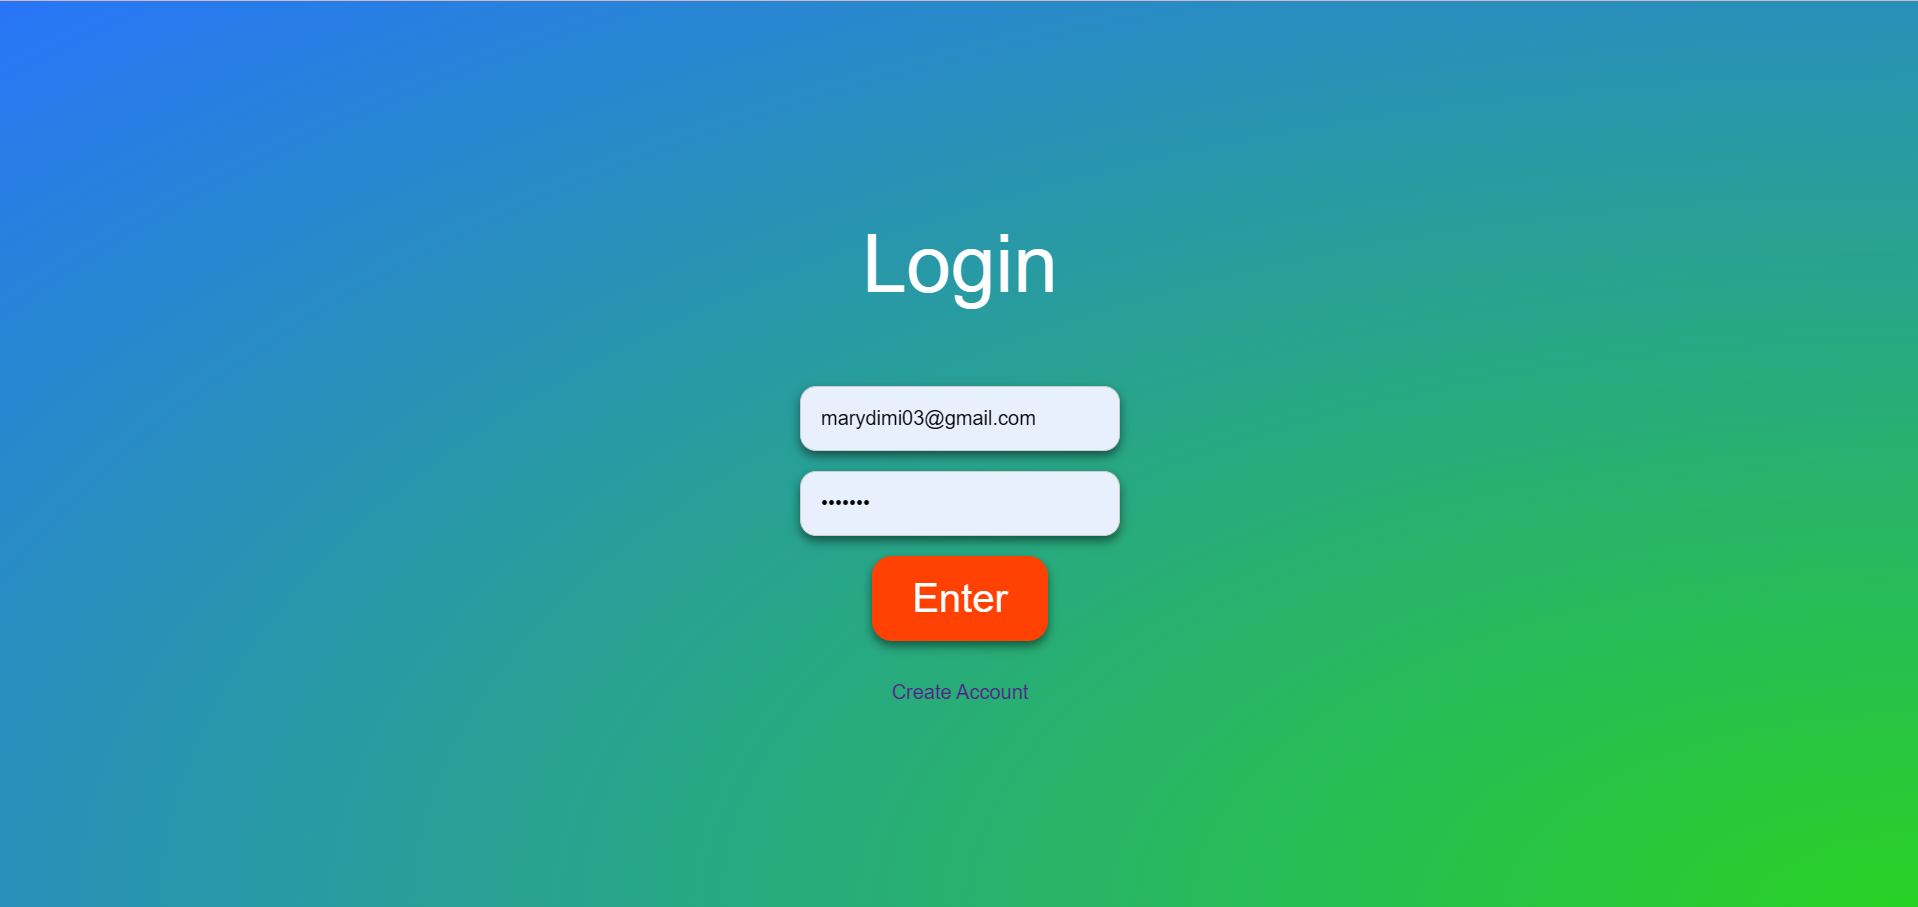
\includegraphics[width=1\linewidth]{img/Login.png}
        \caption{\textlatin{Login Page}}
\end{figure}
\begin{figure}[H]
    \centering
    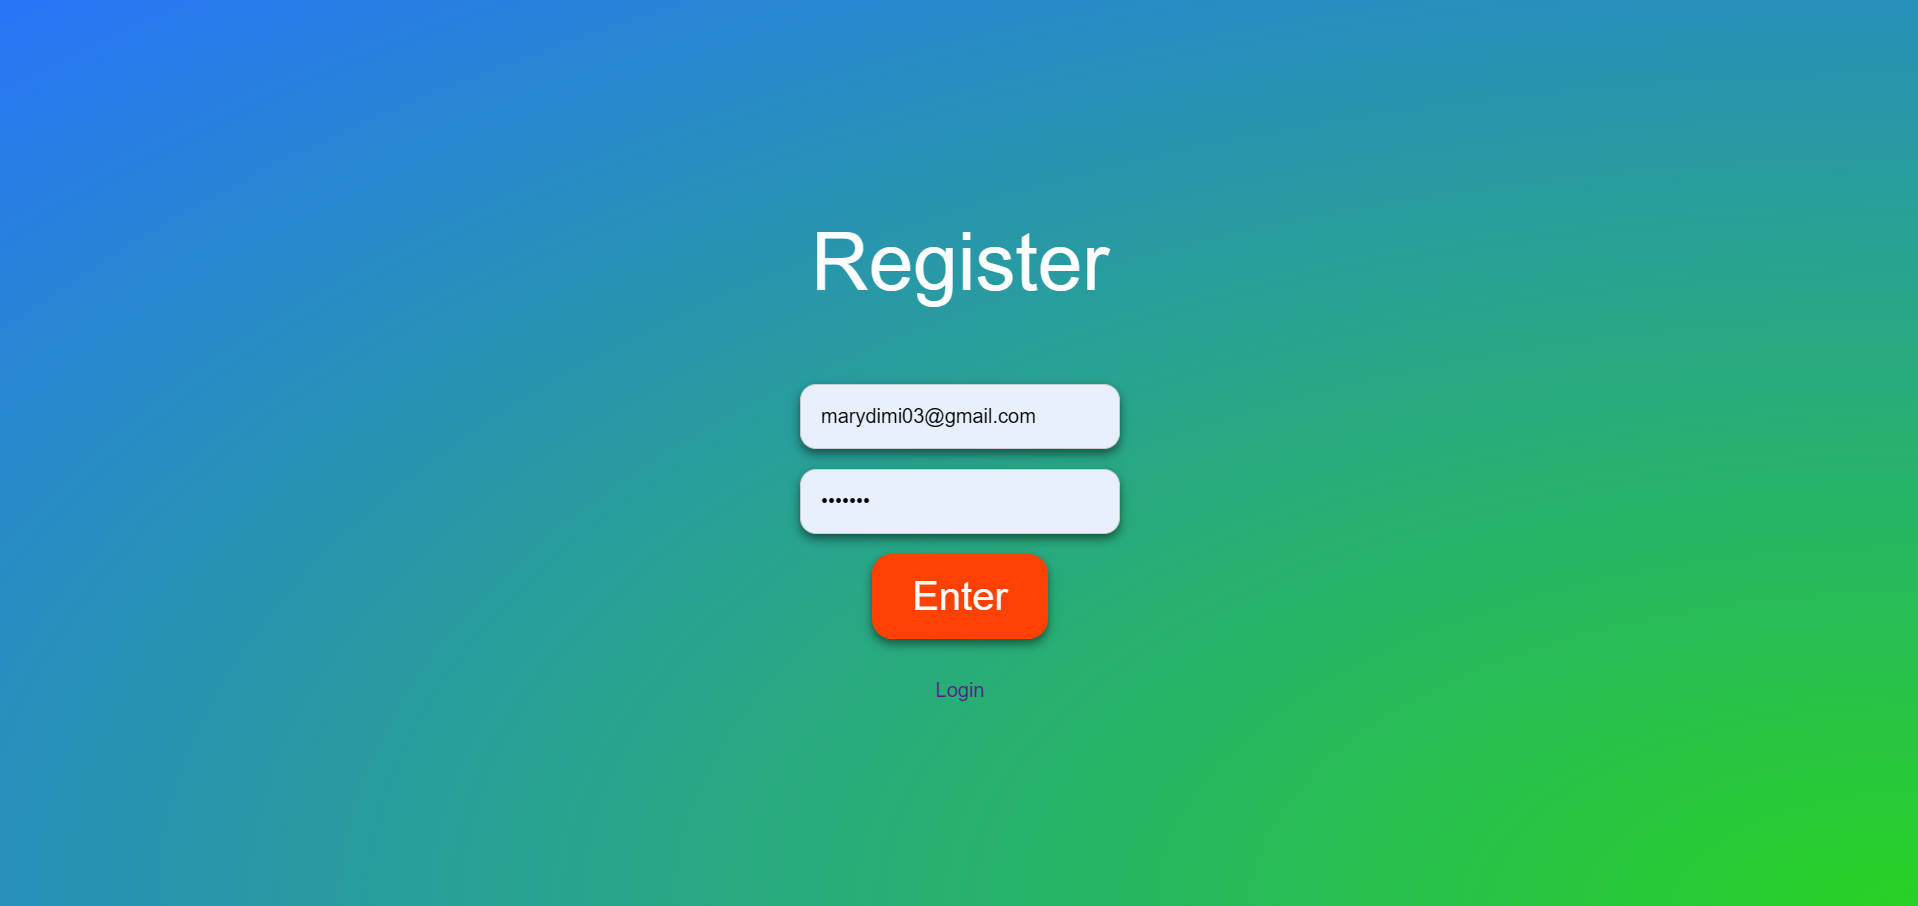
\includegraphics[width=1\linewidth]{img/Register.png}
    \caption{\textlatin{Register Page}}
\end{figure}

\begin{itemize}
    \item Στην συνέχεια θα ακολουθεί το \textbf{κεντρικό μενού,} με τις επιλογές να αρχίσει ή να συνεχίσει την πρόοδο του (\textbf{\textlatin{Learn/Continue}}), εφόσον το λογισμικό θα "θυμάται" που έχει μείνει ο κάθε μαθητής, θα μπορεί να προσπελάσει την λίστα όπου θα φαίνονται όλα τα διαθέσιμα κεφάλαια (\textlatin{\textbf{Chapters}}) και η τελευταία θα είναι να δει τα στατιστικά του (\textbf{\textlatin{Statistics}}), δηλαδή με πιο απλά λόγια τις επιδόσεις του στις δραστηριότητες που έχει ολοκληρώσει (\textlatin{quizzes, exam}).
\end{itemize}
\begin{figure}[H]
    \centering
    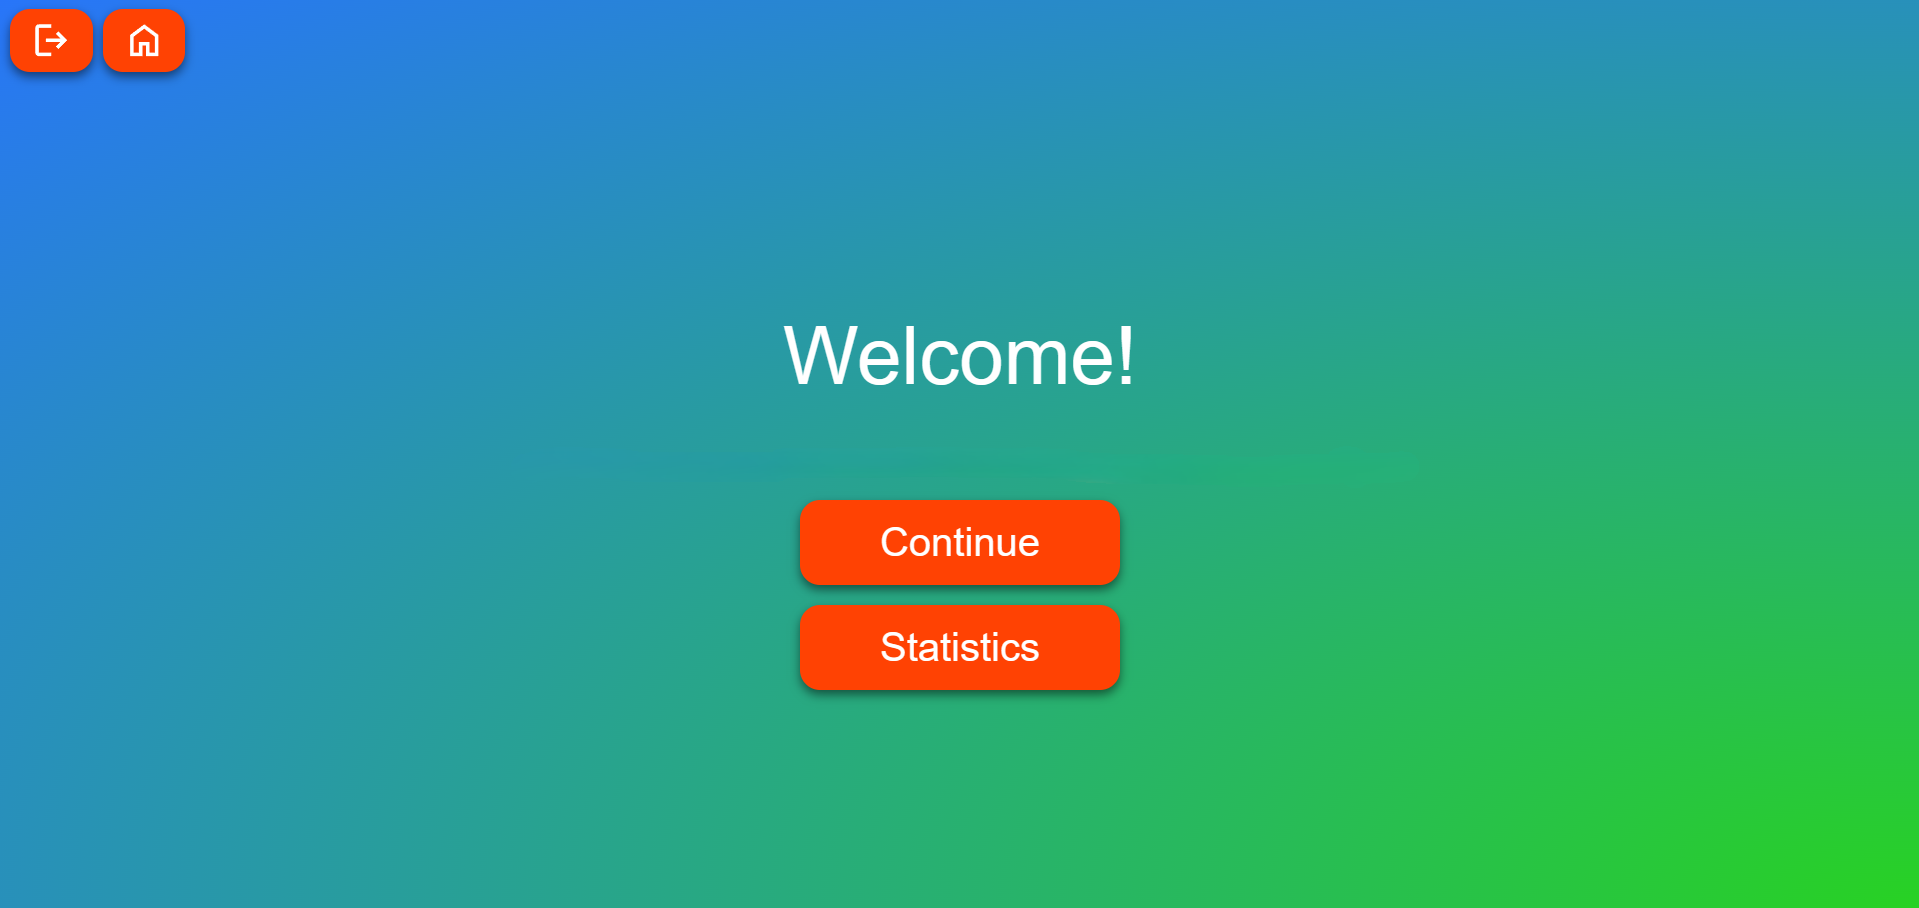
\includegraphics[width=1\linewidth]{img/Menu.png}
    \caption{\textlatin{Menu Page}}
\end{figure}

\begin{itemize}
    \item Παρακάτω βλέπουμε τα κεφάλαια της θεωρίας (\textlatin{\textbf{History, Geography, Culture}}). Ο μαθητής καλείται να τα διαβάσει και να τα αποστηθίσει όσο καλύτερα μπορεί, προκειμένου να βρίσκεται σε θέση να απαντήσει τα \textlatin{quizzes} που ακολουθούν, έπειτα από κάθε κεφάλαιο. Τα κεφάλαια χωρίζονται σε ενότητες με σκοπό την διευκόλυνση του μαθητή κατά την διάρκεια της εκμάθησης τους.
\end{itemize}
\begin{figure}[H]
     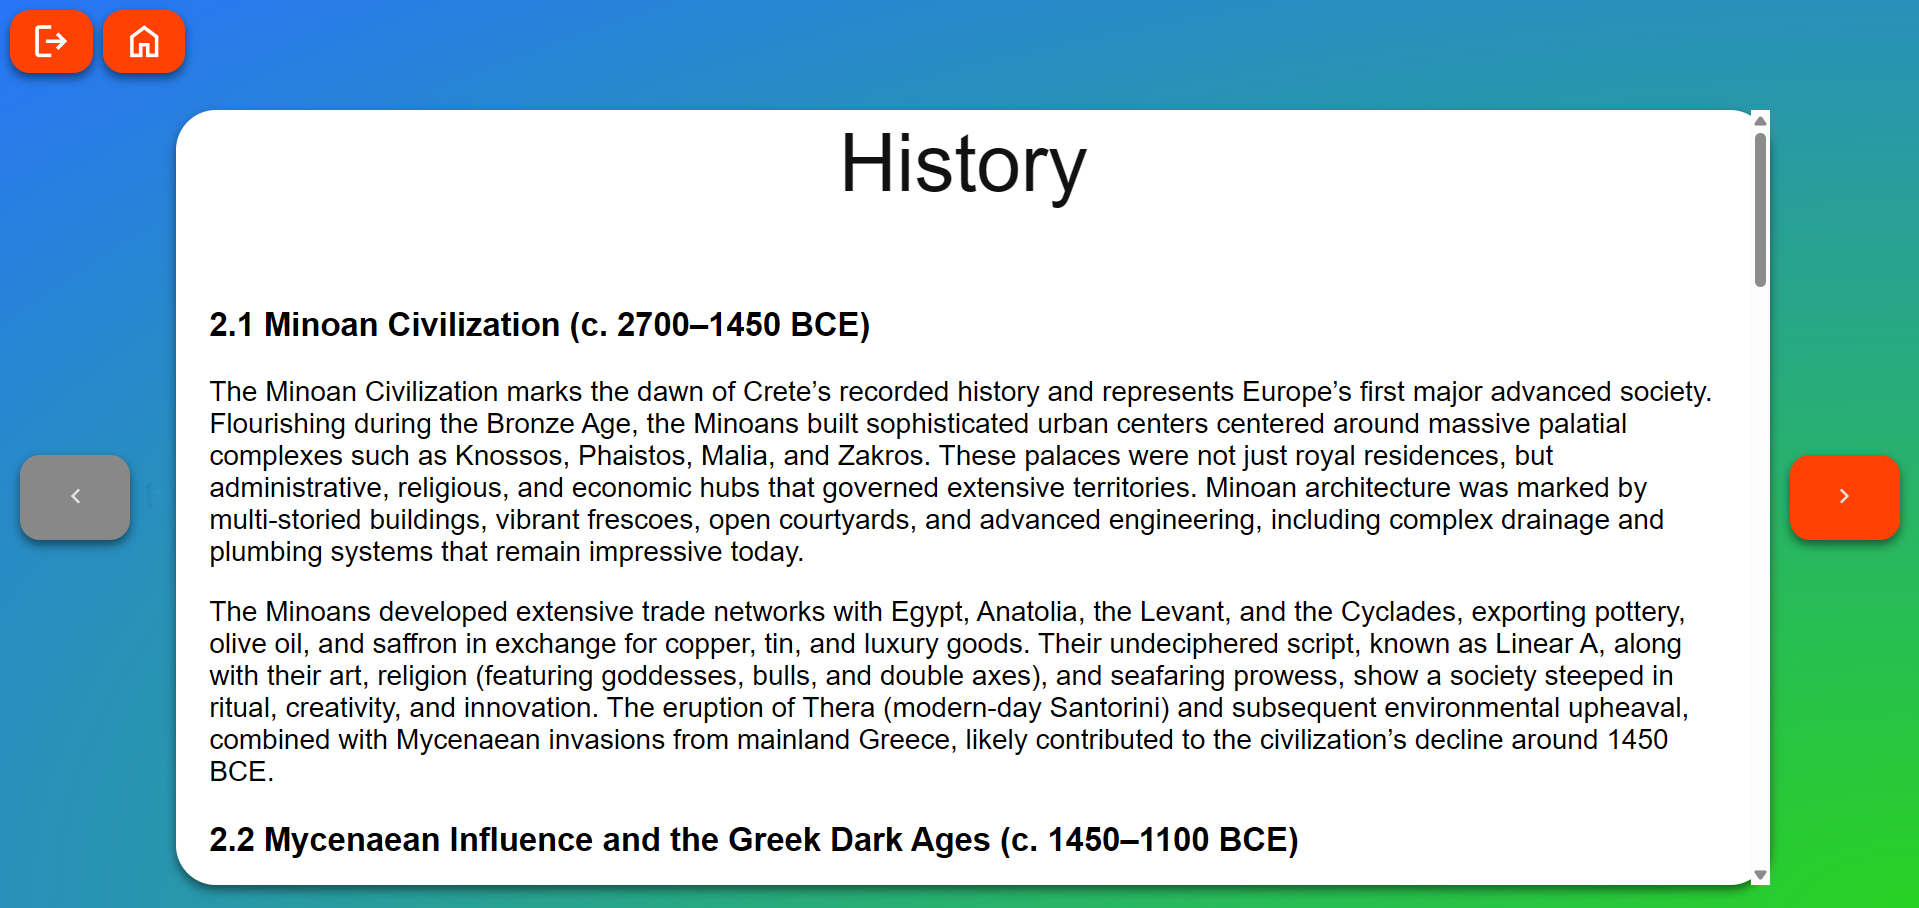
\includegraphics[width=0.5\linewidth]{img/Theory-History.png}
     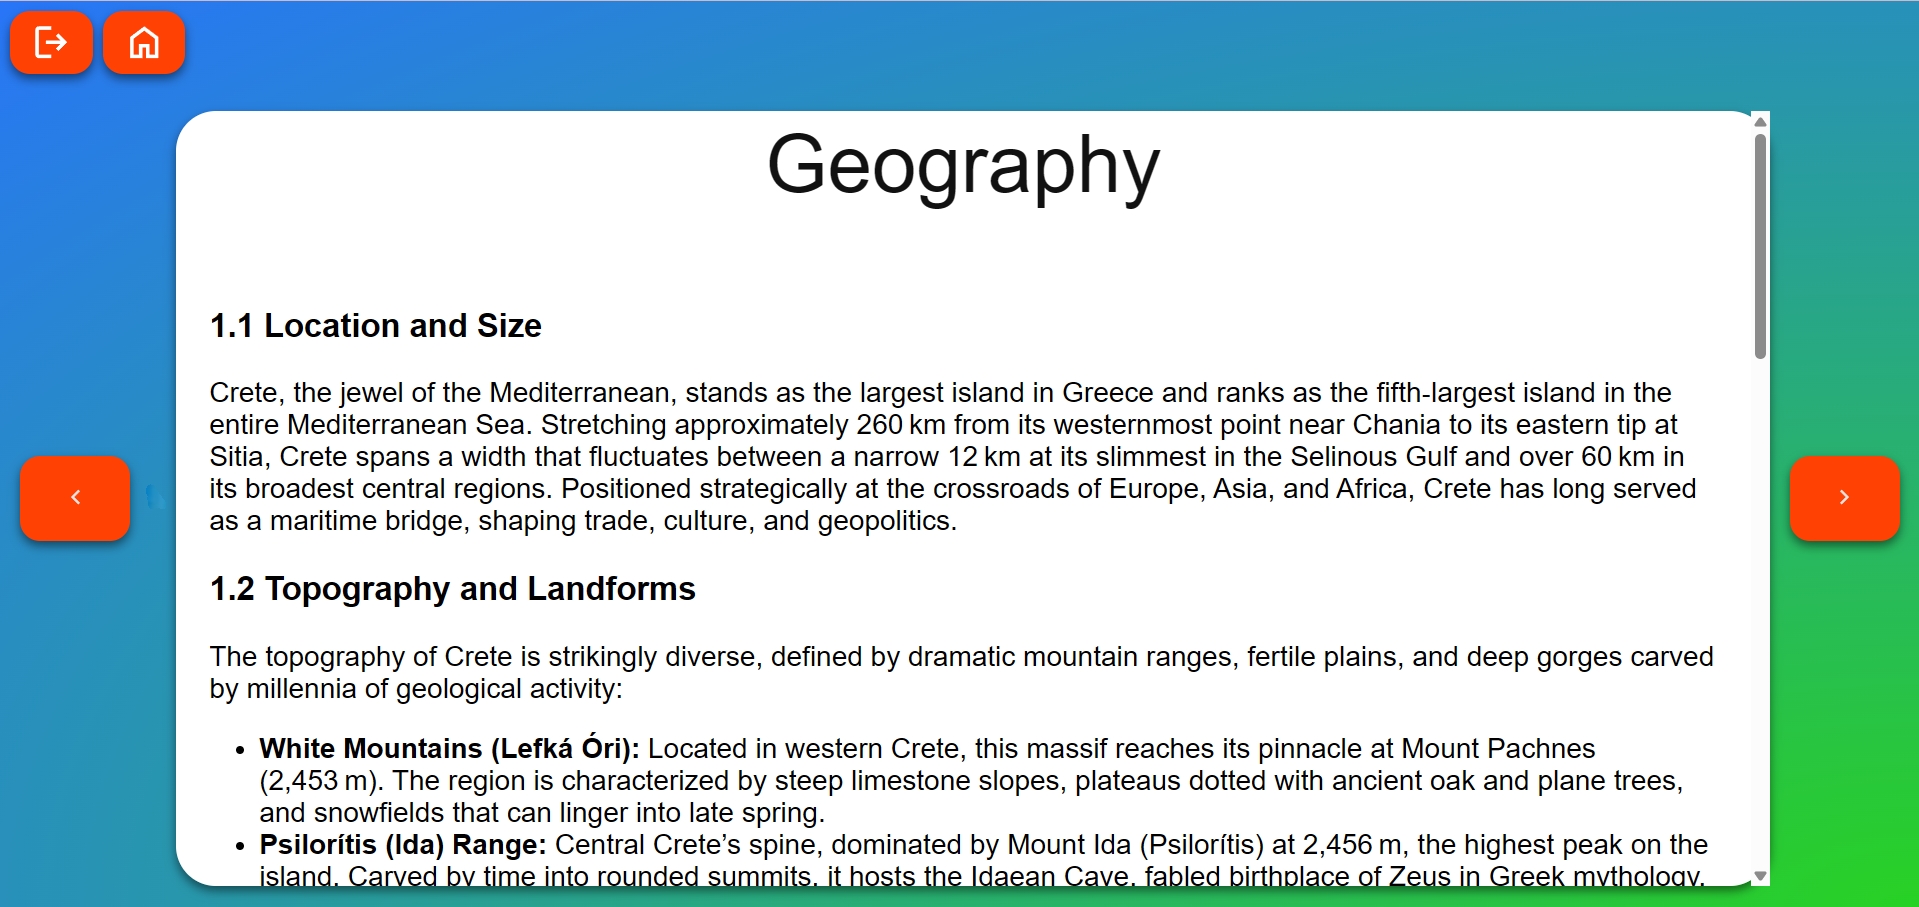
\includegraphics[width=0.5\linewidth]{img/Theory-Geography.png}
\end{figure}
\begin{figure}[H]
    \centering
    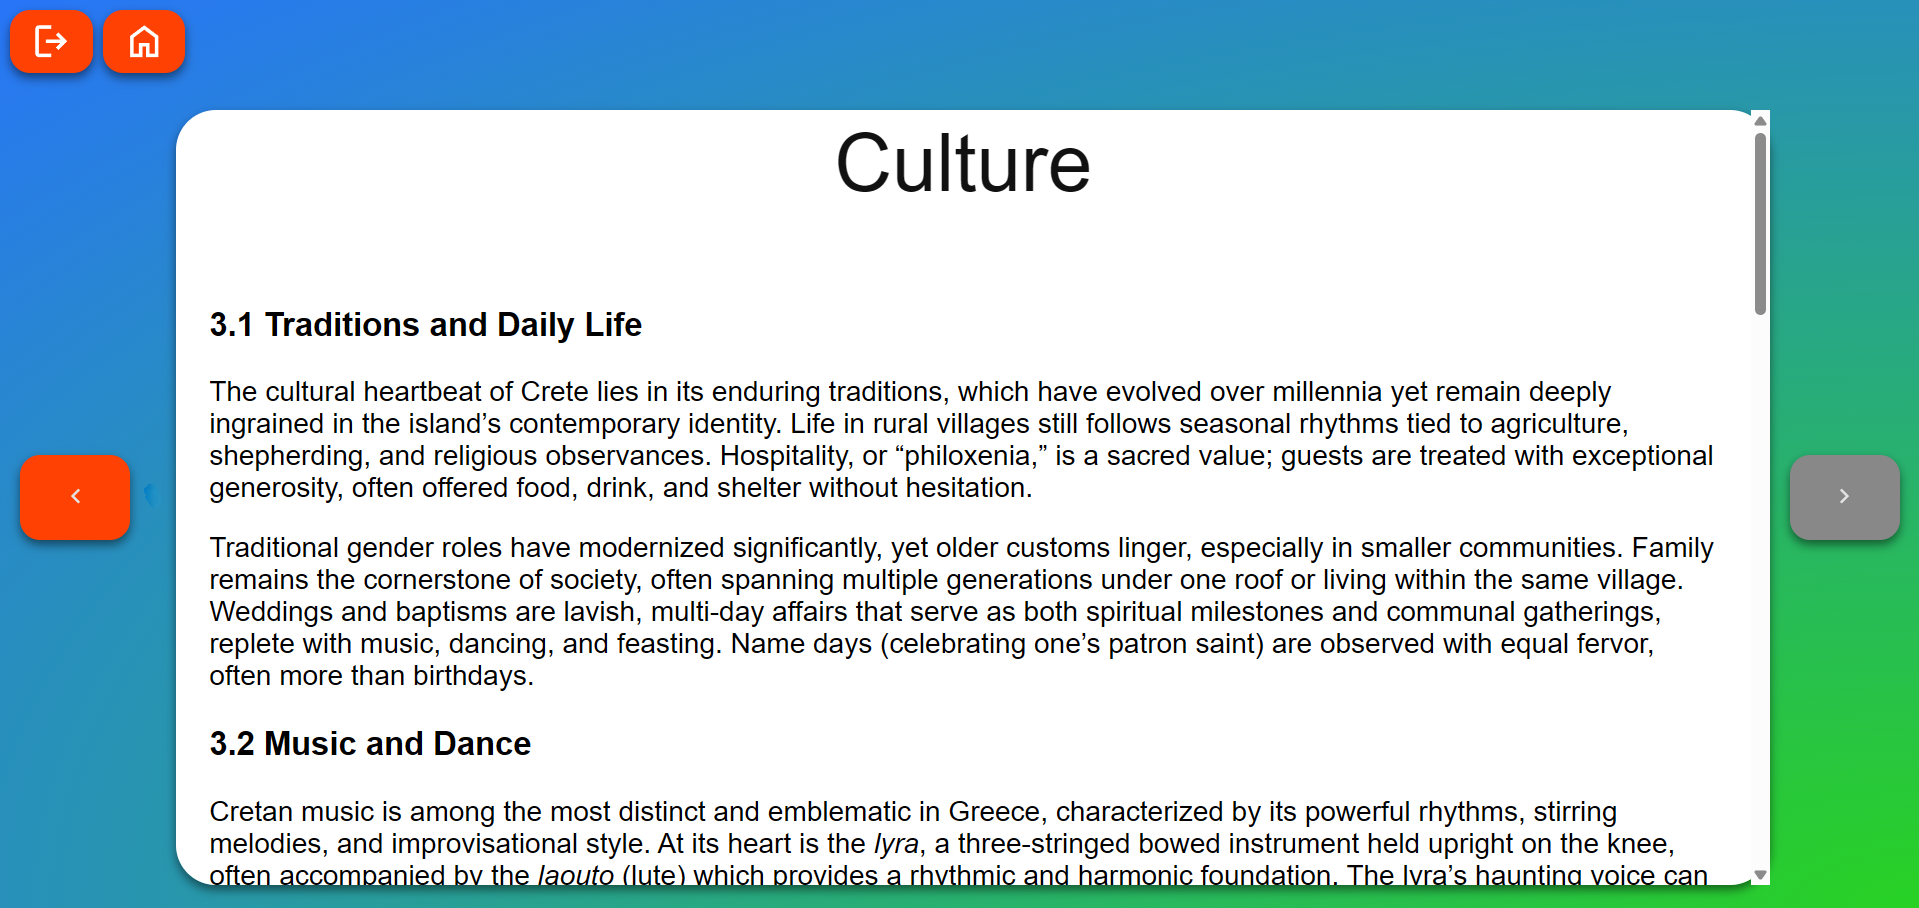
\includegraphics[width=0.5\linewidth]{img/Theory-Culture.png}
    \caption{\textlatin{Theory Chapters Page}}
\end{figure}

\begin{itemize}
    \item Στο τέλος κάθε κεφαλαίου θεωρίας, ο χρήστης θα βρει ένα \textbf{κουμπί \textlatin{"Take the Quiz"}} το οποίο θα τον οδηγήσει στο αντίστοιχο \textlatin{\textbf{quiz}} γνώσεων του συγκεκριμένου κεφαλαίου που βρίσκεται και ολοκλήρωσε. (Κάθε κεφάλαιο έχει από ένα \textlatin{quiz} 15 ερωτήσεων, άρα συνολικά έχουμε 3 \textlatin{quizzes} και 45 διαφορετικές ερωτήσεις).
\end{itemize}
\begin{figure}[H]
    \centering
    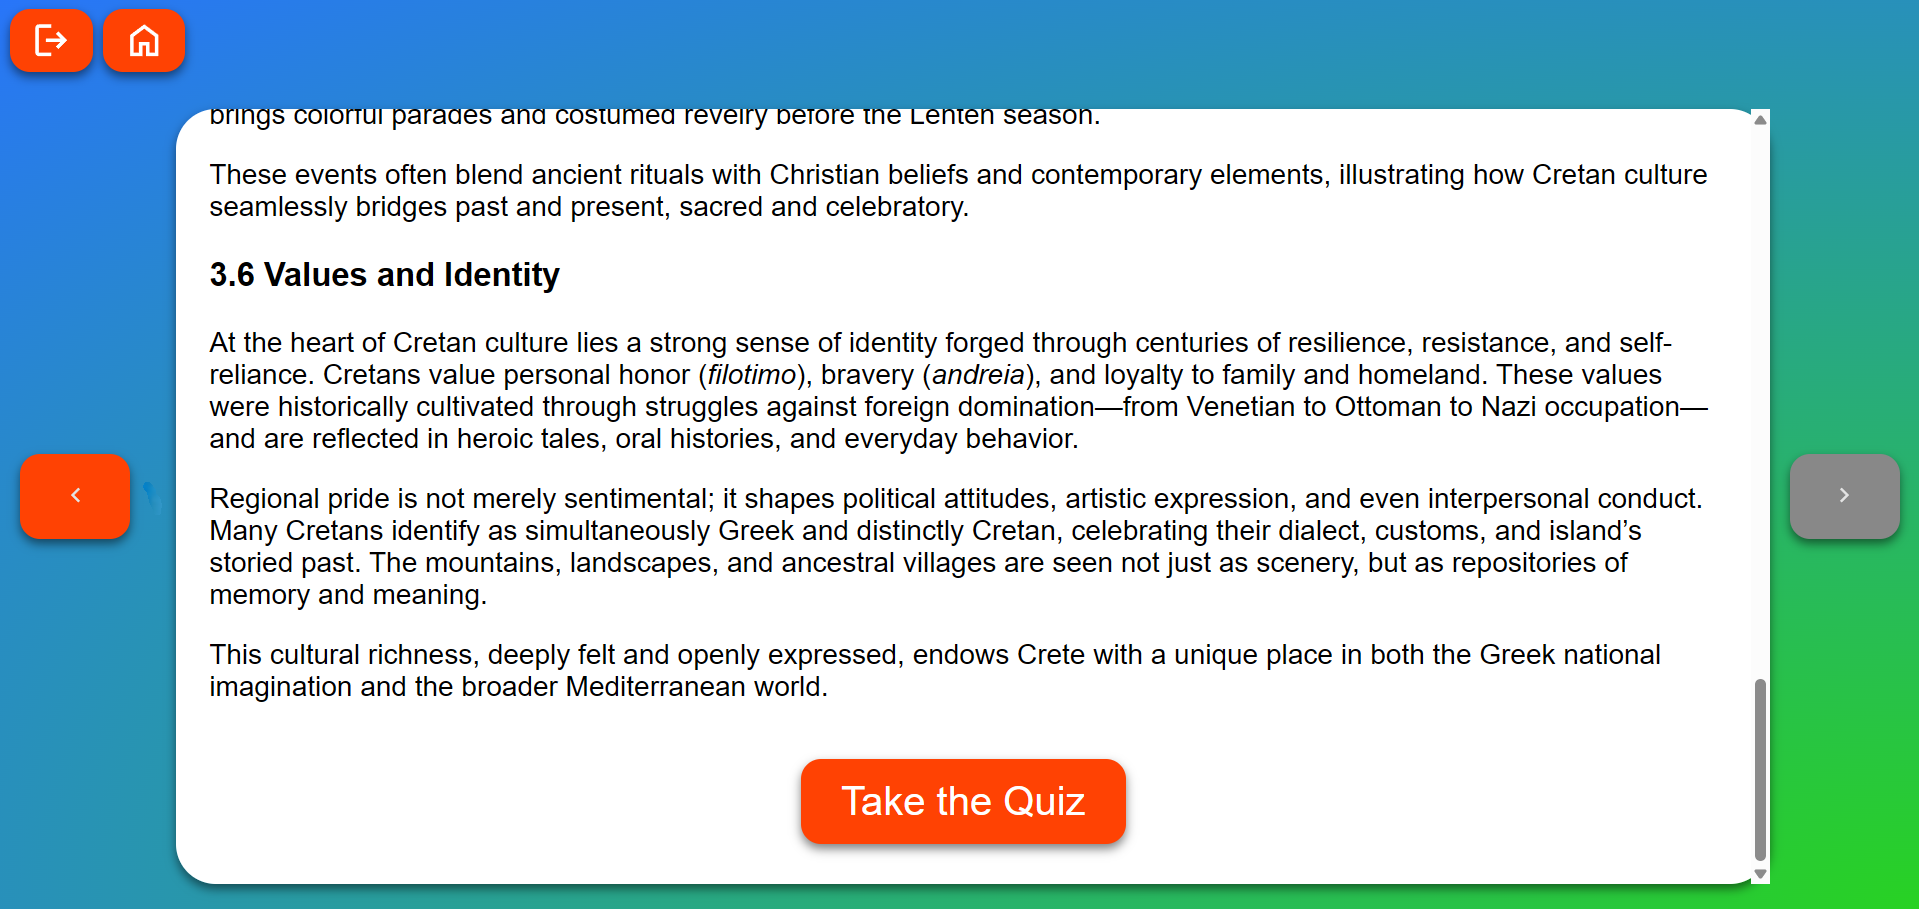
\includegraphics[width=1\linewidth]{img/Theory-TestButton.png}
    \caption{\textlatin{Theory Page-Quiz Button}}
\end{figure}

\begin{itemize}
    \item Αφού ο μαθητής έχει τελειώσει και απαντήσει όλες της ερωτήσεις των τριών κεφαλαίων, τελευταίο βήμα είναι να κάνει το τελικό, επαναληπτικό διαγώνισμα (\textlatin{\textbf{Exam}}), ειδικά προσαρμοσμένο πάνω στις γνώσεις, στις αδυναμίες και στις ικανότητες του κάθε μαθητή.
\end{itemize}

\begin{figure}[H]
    \centering
    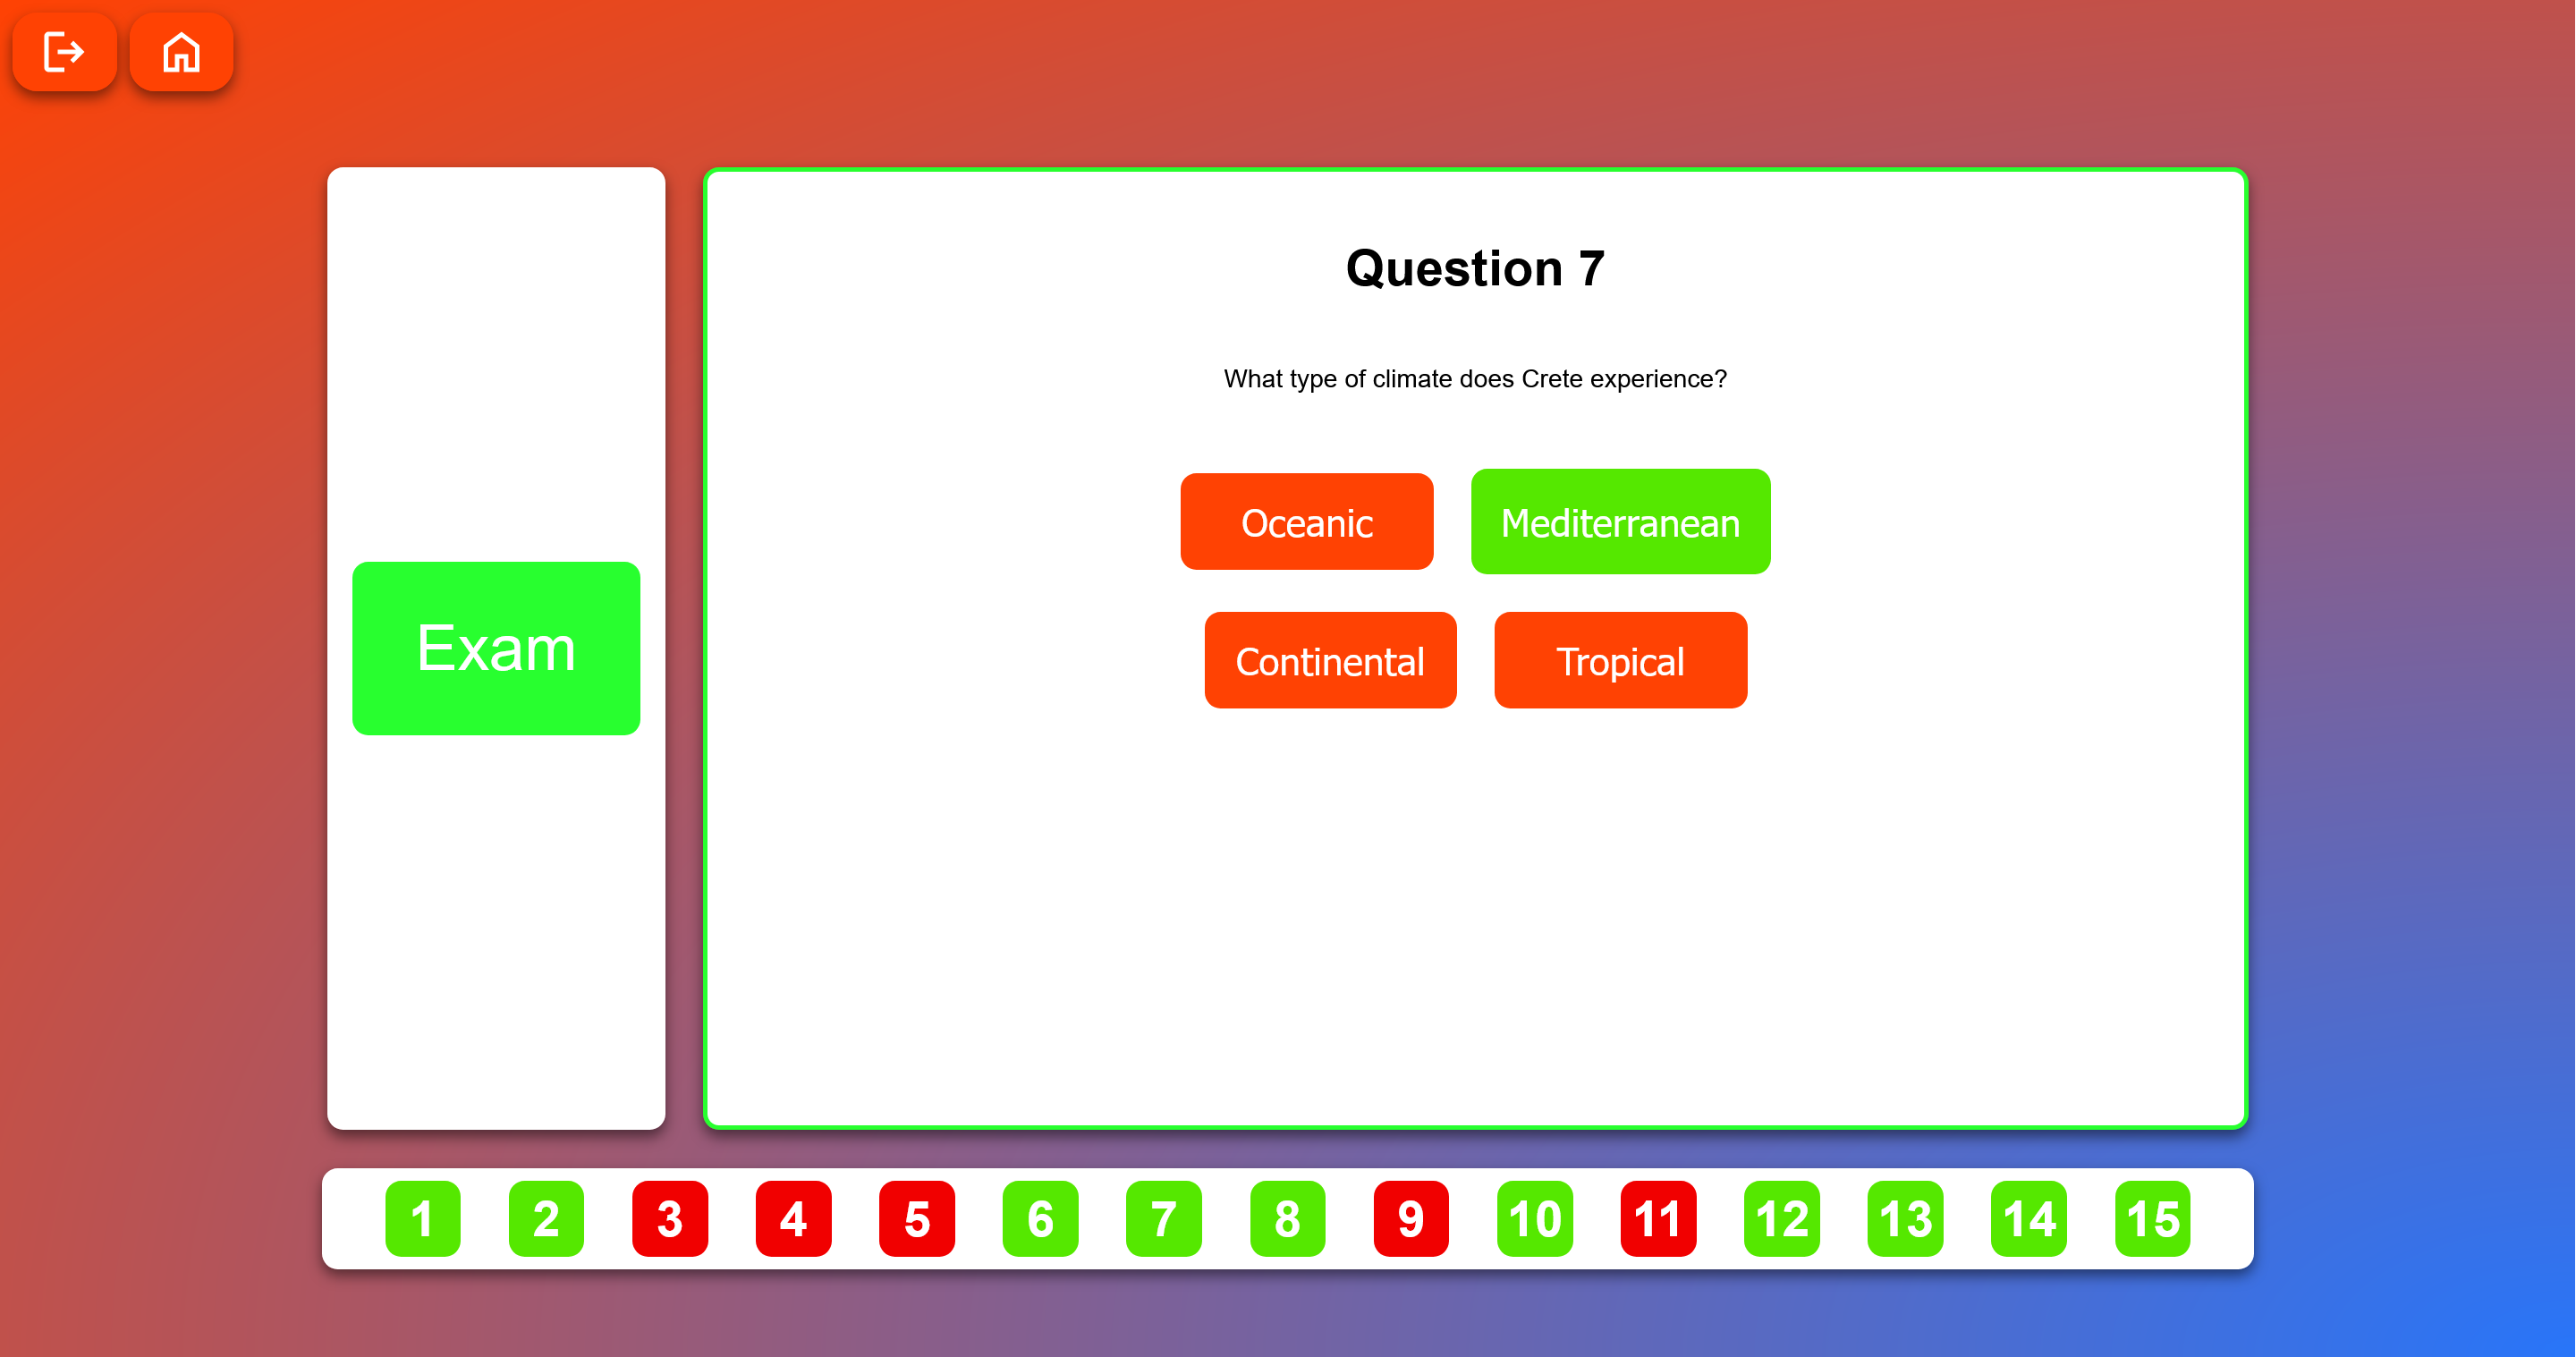
\includegraphics[width=1\linewidth]{img/ExamQuiz.png}
    \caption{\textlatin{Exam Page}}
\end{figure}

\begin{itemize}
    \item Βέβαια, πριν το τελικό \textlatin{Exam}, θα προτείνεται στον μαθητή \textbf{έξτρα προσαρμοσμένο υλικό (\textlatin{Review})}, σύμφωνα με τις επιδόσεις του στα \textlatin{Quizzes}, εάν αυτό κρίνεται απαραίτητο (δηλαδή εάν το σκορ του μαθητή είναι χαμηλό).
\end{itemize}
\begin{figure}[H]
    \centering
    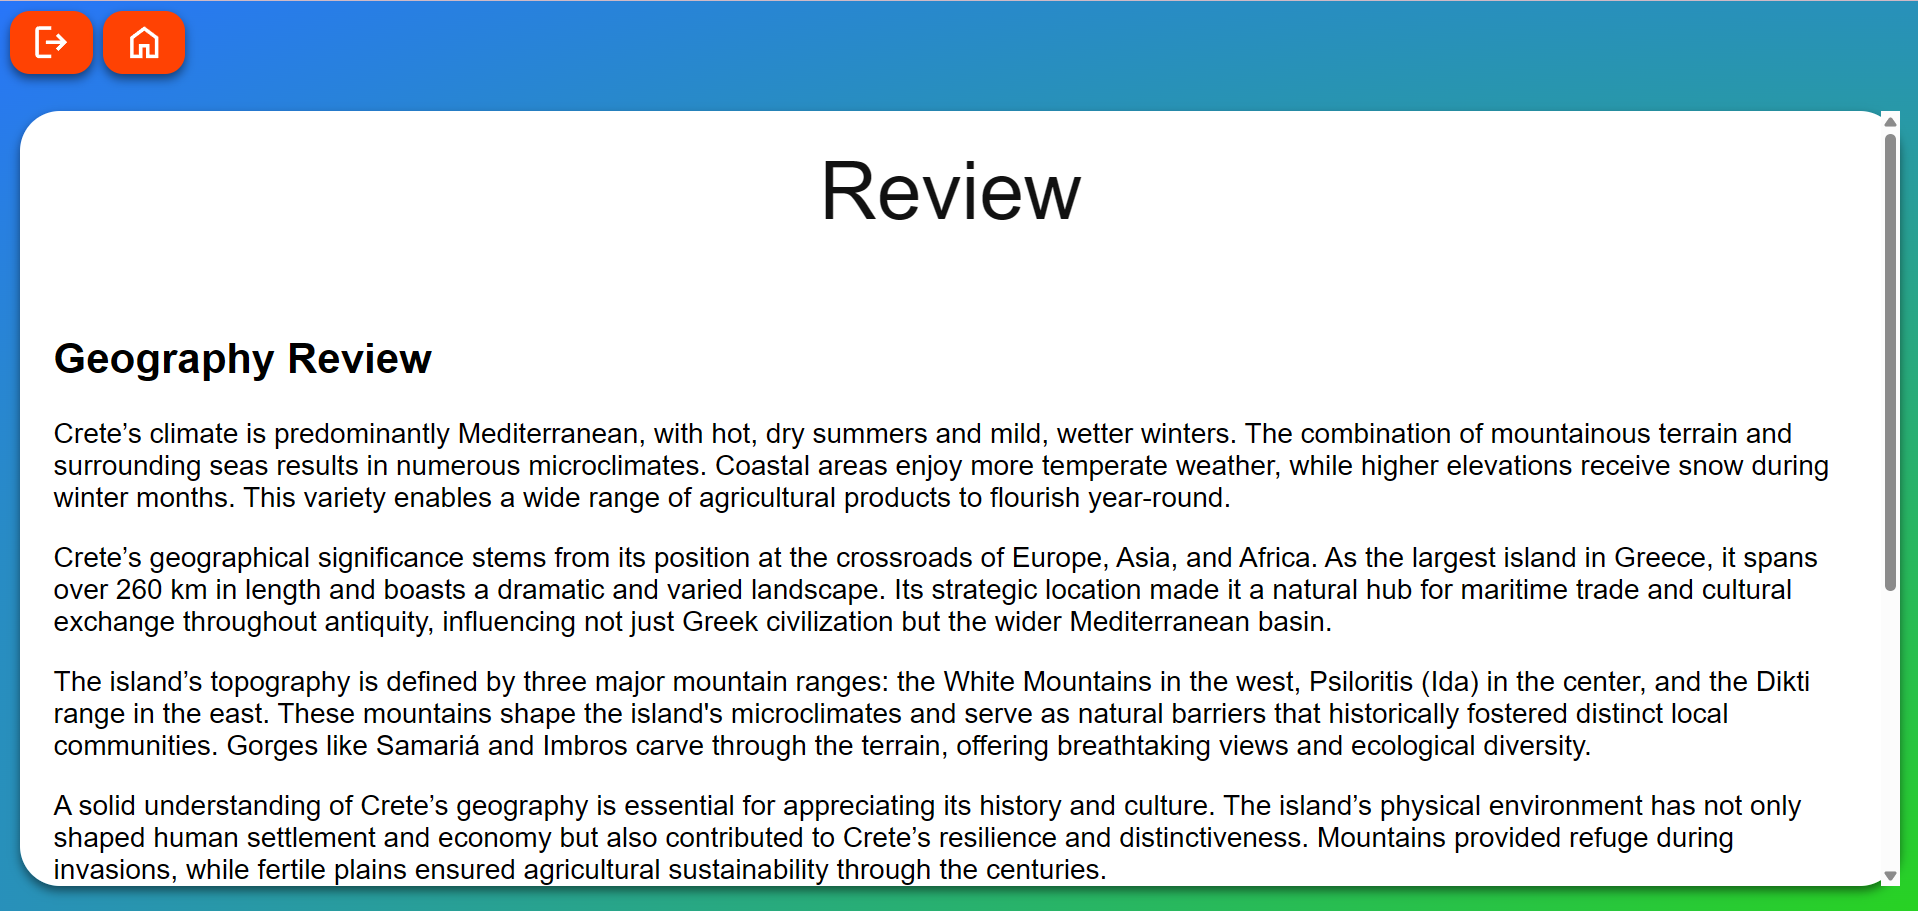
\includegraphics[width=1\linewidth]{img/Review.png}
    \caption{\textlatin{Review Page}}
\end{figure}



\begin{itemize}
    \item Ο μαθητής, θα έχει επίσης την δυνατότητα, να επισκέπτεται όσες φορές θέλει το κομμάτι της θεωρίας που επιθυμεί να επαναλάβει, έτσι ώστε να μάθει σε μεγαλύτερο βάθος και να προσαρμοστεί όσο καλύτερα γίνεται στα κεφάλαια μέσω \textlatin{\textbf{Chapters}}. Ακόμα, θα μπορεί να δει πόσες και ποιες ερωτήσεις έχει απαντήσει σε κάθε ένα από τα κεφάλαια ώστε να έχει μία "καθαρή" εικόνα της προόδου του.
\end{itemize}
\begin{figure}[H]
    \centering
    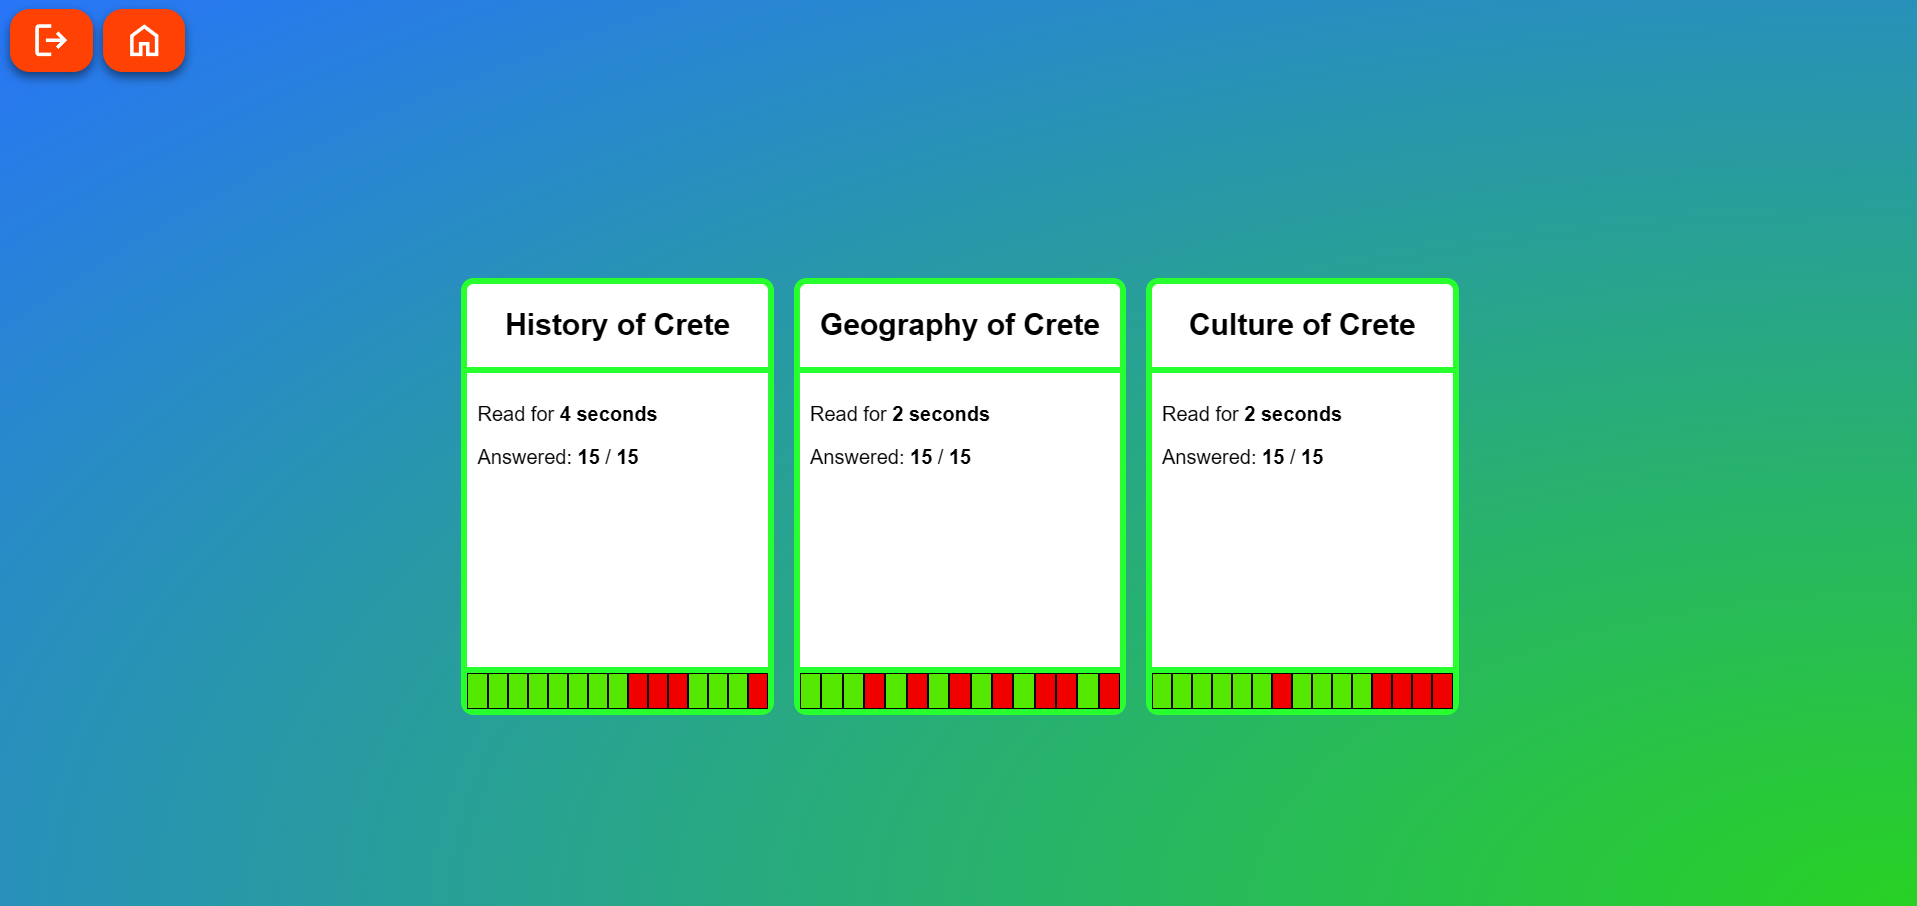
\includegraphics[width=1\linewidth]{img/Chapter-Progress.png}
    \caption{\textlatin{Chapter Progress Page}}
\end{figure}

\begin{itemize}
    \item Όσον αφορά το τμήμα των \textbf{Στατιστικών}, εκεί ο μαθητής θα έχει την δυνατότητα να ενημερώνεται για την πρόοδο του, τον χρόνο που καταναλώνει στα \textlatin{quizzes} και στο \textlatin{Exam} και συνεπώς να εντοπίζει τα πεδία στα οποία χρειάζεται περισσότερη μελέτη, με σκοπό την αυτοβελτίωσή του και την καλύτερη κατανόηση της ύλης. Τα γραφήματα θα στηρίζονται στην συνολική του εικόνα/ απόδοση, με γνώμονα κάθε κεφάλαιο ξεχωριστά και τέλος συγκεκριμένα για κάθε ερώτηση.
\end{itemize}
\begin{figure}[H]
    \centering
    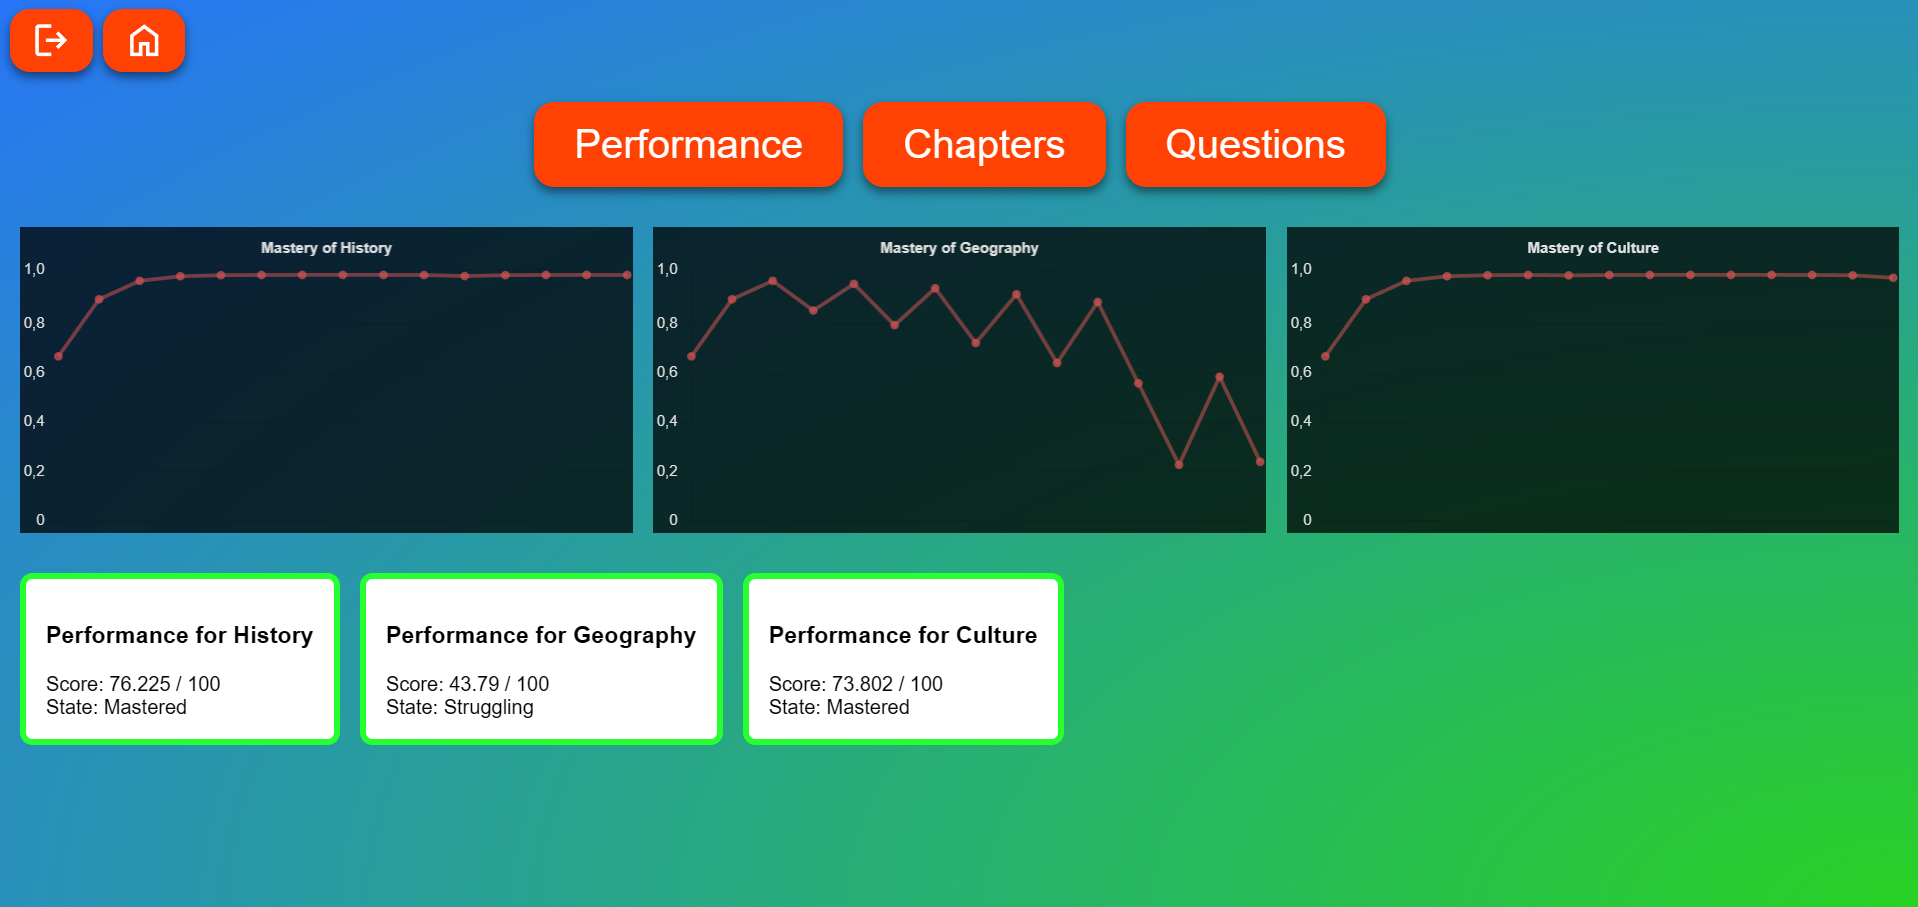
\includegraphics[width=0.5\linewidth]{img/Statistics.png}
    \caption{\textlatin{Statistics Page (Performance}}
\end{figure}
\begin{figure}[H]
    \centering
    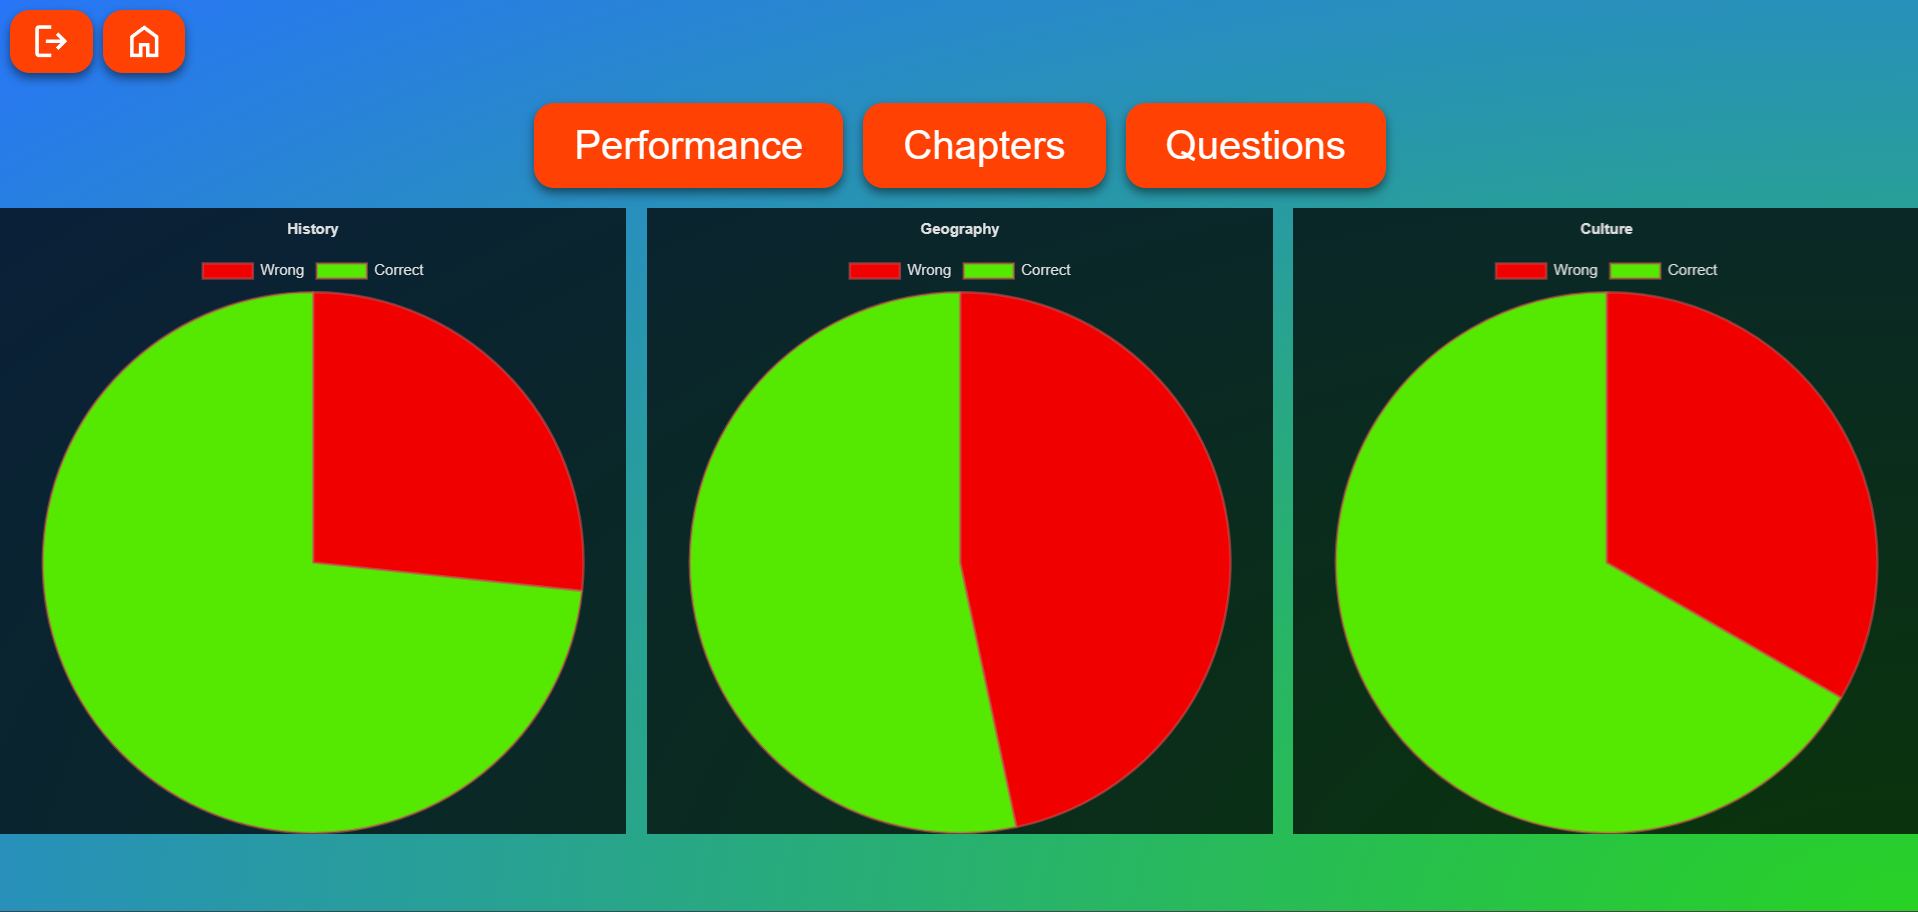
\includegraphics[width=0.5\linewidth]{img/Statistics-Quests.png}
    \caption{\textlatin{Statistics Page (Questions)}}
\end{figure}

\bibliographystyle{alpha}
\bibliography{chrono_bibliography}

\end{document}